\chapter{Resultados y discusión}
En este capítulo se presentan los resultados obtenidos de las simulaciones de transmisión de calor por conducción de un sistema TPV de un nano-espaciador y
radiación por campo cercano entre dos placas paralelas a 800°C el emisor y 25°C la célula. A su vez se representa las relaciones entre la potencia radiada vs la potencia conducida por cantidad de espaciadores y por distancia de separación en un sistema de emisor y célula de 1cm2.
\begin{itemize}
	\item Primero se comprueba si el procedimiento de extracción de datos de la simulación de transmisión de calor por conducción en CFD es adecuado y no presenta un error relativo significativo respecto a la teoría.
	\item Se presentan los resultados de las simulaciones de transmisión de calor por conducción y por radiación de campo cercano para diferentes combinaciones de materiales de emisor y célula, y la relación entre ambas simulaciones.
	\item Se estudia el número mínimo de espaciadores necesarios para soportar la carga de los emisores.
	\item Por último, se presentan los resultados de usar un nano-espaciador de $Si$ en vez de $SiO_2$ para emisores de $Si$ y $SS$.
\end{itemize}
%% COMPROBACIÓN DEL PROCEDIMIENTO DE EXTRACCIÓN DE RESULTADOS DE CFD
\section{Comprobación del procedimiento de extracción de resultados de CFD}
El procedimiento de extracción de resultados de CFD está definido en el punto \ref{it:extraerResCFD} del capítulo \ref{chapter:Metodos} y para su comprobación se procede a realizar una simulación en CFD donde el emisor y la célula son de $Si$ y el nano-espaciador de $SiO_2$ con las características constantes a 25\textdegree C, con la base cuadrada de 1 $mm^2$ y la altura del nano-espaciador a unos 1000nm, todo con la escalas correspondientes aplicadas.\\\\
La conductividad térmica ($\sigma$) del $Si$ es 182.977 W/m\textdegree C y la del $SiO_2$ es 1.30067 W/m\textdegree C ambas a 25\textdegree C. De la simulación se extrae que el flujo de calor del sistema y la temperatura media máxima y mínima de las superficies de contacto del nano-espaciador con los otros componentes del sistema.\\\\
La temperatura media máxima del nano-espaciador es 792.601\textdegree C, la temperatura media mínima del nano-espaciador es 32.3903\textdegree C y el flujo de calor es 0.00889793 W. Con los resultados de las temperaturas medias del nano-espaciador se obtiene un flujo de calor teórico de 0.00889905 W, obteniéndose un error relativo aproximado del 0.0126\%, por lo tanto el procedimiento es apropiado para la obtención de los resultados de las simulaciones de transmisión de calor por conducción.
%%% SIMULACIONES DE TRANSMISIÓN DE CALOR POR CONDUCCIÓN EN CFD
\section{Sistema TPV de Si-SiO2-Si}
El sistema TPV a estudiado está compuesto de un emisor de $Si$ a 800\textdegree C, una nano-espaciador de $SiO_2$ y una célula de $Si$ a 25\textdegree C. Se estudia el efecto de la porosidad del $SiO_2$ en la potencia de conducción total que fluye por un nano-espaciador de diferentes alturas, el efecto de la resistencia de contacto sobre la conductividad del sistema y la relación entre la potencia radiada y conducida para cada caso en el rango de longitudes de onda que trabaja la célula.\\\\
\begin{figure}[H]
	\centering
	\begin{subfigure}[b]{0.49\textwidth}
		\centering
		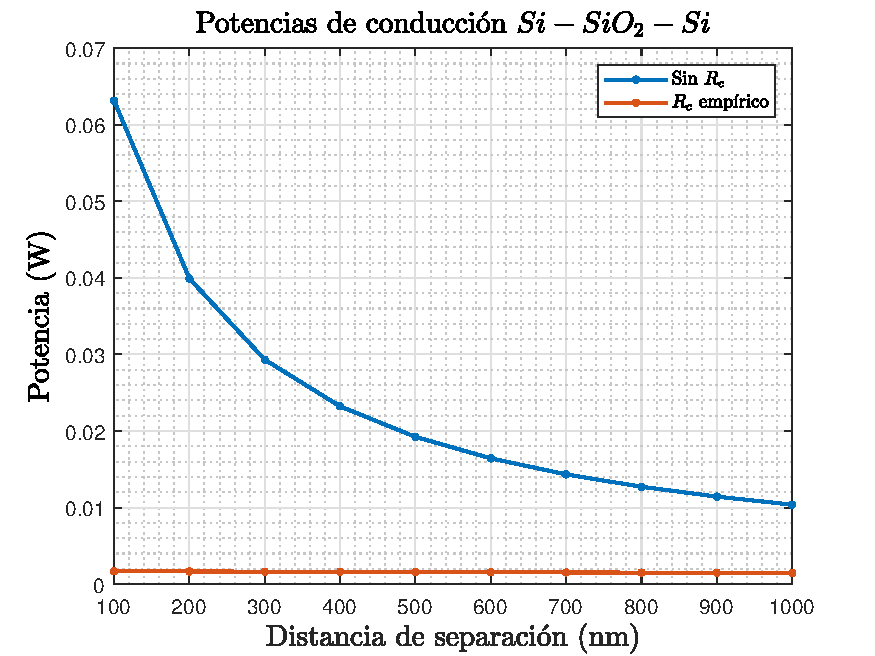
\includegraphics[width=1.0\textwidth]{figuras/Resultados/conduccion/pdf/Prc_SiSiO2Si.pdf}
		\caption{ }
		\label{fig:Prc_SiSiO2Si}
	\end{subfigure}
	\begin{subfigure}[b]{0.49\textwidth}
		\centering
		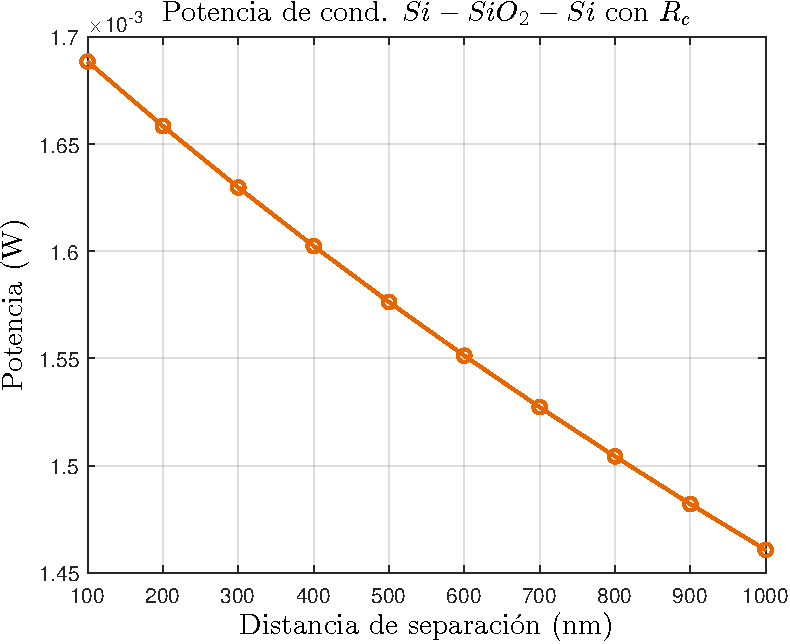
\includegraphics[width=1.0\textwidth]{figuras/Resultados/conduccion/pdf/Prc2_SiSiO2Si.pdf}
		\caption{ }
		\label{fig:Prc2_SiSiO2Si}
	\end{subfigure}
	\begin{subfigure}[b]{0.49\textwidth}
		\centering
		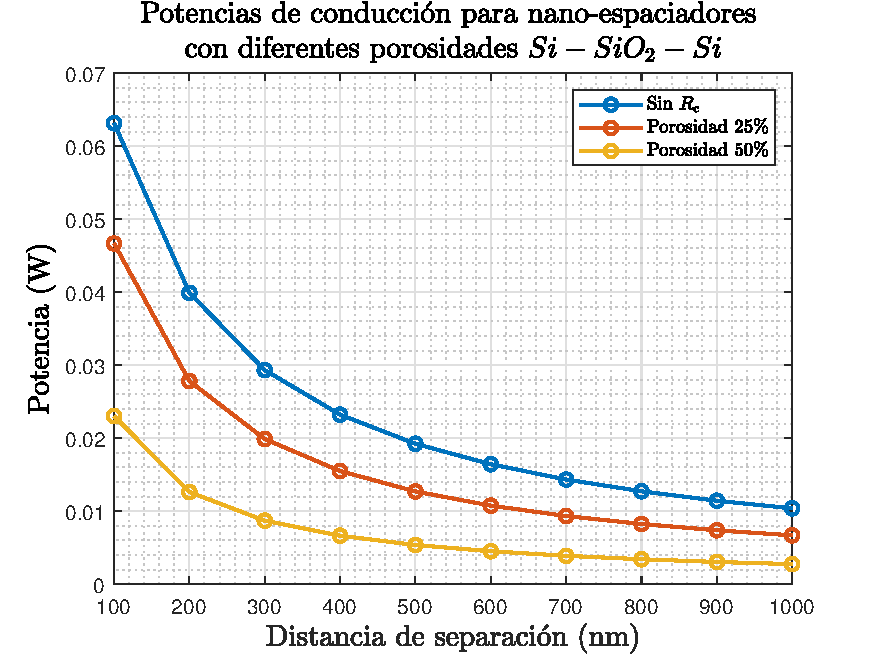
\includegraphics[width=1.0\textwidth]{figuras/Resultados/conduccion/pdf/Ppor_SiSiO2Si.pdf}
		\caption{ }
		\label{fig:Ppor_SiSiO2Si}
	\end{subfigure}
	\begin{subfigure}[b]{0.49\textwidth}
		\centering
		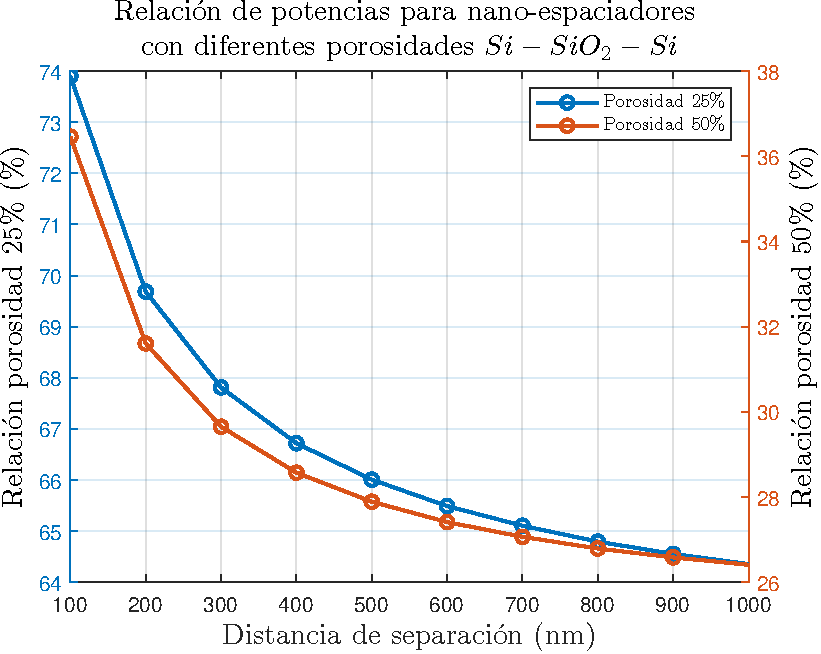
\includegraphics[width=1.0\textwidth]{figuras/Resultados/conduccion/pdf/relPpor_SiSiO2Si.pdf}
		\caption{ }
		\label{fig:relPpor_SiSiO2Si}
	\end{subfigure}
	\caption{ }
	\label{fig:Potencias_SiSiO2Si}
\end{figure}
\[Rel=\frac{\left| P_{Porosidad}- P_{Normal} \right|}{P_{Normal}}\cdot 100\]
\[P(d,p1(p),q1(p))=\frac{p1(p)}{d+q1(p)}\]
\[p1(p)=-16.47\cdot p +11.03 \ q1(p)=-106.80\cdot p+74.68\]
\[P(d,p)=\frac{  16.47\cdot p-11.03 }{d-106.80\cdot p +74.68}\]
\subsection{Efectos de la resistencia de contacto}

De las simulaciones de transmisión de calor de CFD, se obtienen los siguientes resultados:
\begin{table}[H]
	\centering
		\begin{tabular}{|c||c|c|c|c||c|c|}
		\hline
			\multirow{2}{*}{ }& \multicolumn{6}{c|}{\textbf{\large Potencias según como se transmite el calor}}\\ \cline{2-7}
		  & \multicolumn{4}{c||}{Conducción (W/nº nano-espaciadores)}& \multicolumn{2}{c|}{Radiación $(W/m^2)$}\\ \hline
			Dist. (nm)&$P_{Normal}$&$P_{R_c-Empirico}$&$P_{Porosidad25}$&$P_{Porosidad50}$&$P_{Eg>0.7eV}$&$P_{full}$\\ \hline \hline
			100&6,31E-02&1,69E-03&4,67E-02&2,30E-02&5,07E+03&1,65E+05\\ \hline
			200&3,99E-02&1,66E-03&2,78E-02&1,26E-02&3,11E+03&1,10E+05\\ \hline
			300&2,93E-02&1,63E-03&1,99E-02&8,69E-03&2,30E+03&8,51E+04\\ \hline
			400&2,32E-02&1,60E-03&1,55E-02&6,63E-03&1,90E+03&7,01E+04\\ \hline
			500&1,92E-02&1,58E-03&1,27E-02&5,36E-03&1,70E+03&6,02E+04\\ \hline
			600&1,64E-02&1,55E-03&1,08E-02&4,50E-03&1,66E+03&5,32E+04\\ \hline
			700&1,43E-02&1,53E-03&9,33E-03&3,88E-03&1,72E+03&4,80E+04\\ \hline
			800&1,27E-02&1,50E-03&8,24E-03&3,41E-03&1,82E+03&4,43E+04\\ \hline
			900&1,14E-02&1,48E-03&7,38E-03&3,04E-03&1,86E+03&4,14E+04\\ \hline
			1000&1,04E-02&1,46E-03&6,68E-03&2,74E-03&1,80E+03&3,93E+04\\ \hline
		\end{tabular}
	\caption{Tabla de resultados de las simulaciones de conducción y radiación de campo cercano para diferentes alturas del nano-espaciador. Flujos de calor del TPV $Si-SiO_2-Si$ para diferentes alturas del nano-espaciador y para los casos sin $R_c$, con $R_c$ de \cite{nf_TPV_Pillars_SiO2}, sin $R_c$ pero con las proporciones de las porosidades de \cite{ThermalConductivity_SiO2_2018} para un 25\% y un 50\%.}
	\label{tab:condTerSiSiO2Si}
\end{table}



\subsection{Efectos de la porosidad}

\subsection{Relación entre conducción y radiación}

\section{Caso 2: Sistema TPV de $Si-SiO_2-Ge$}

\section{Caso 3: Sistema TPV de $SS-SiO_2-Ge$}

\section{Caso 4: Sistema TPV de $SiC-SiO_2-Ge$}

\section{Resultados}


\section{Discusión}